% FILE: figures/bkt_transition.tex
% BKT-like vortex/antivortex schematic

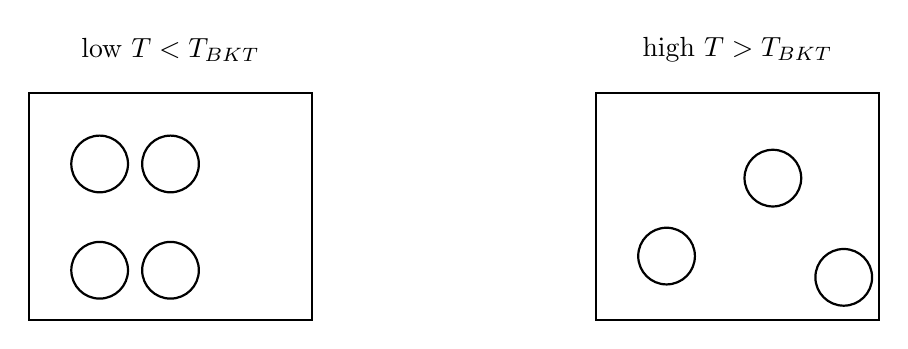
\begin{tikzpicture}[>=latex,thick,scale=0.9]
  % Low T panel
  \node[anchor=south] at (-4,3.3) {low $T<T_{\text{BKT}}$};
  \draw (-6,-0.2) rectangle (-2,3);

  % Bound vortex-antivortex pairs
  \draw[->] (-5,0.5) circle (0.4);
  \draw[<-] (-4,0.5) circle (0.4);
  \draw[->] (-5,2.0) circle (0.4);
  \draw[<-] (-4,2.0) circle (0.4);

  % High T panel
  \node[anchor=south] at (4,3.3) {high $T>T_{\text{BKT}}$};
  \draw (2,-0.2) rectangle (6,3);

  % Free vortices
  \draw[->] (3,0.7) circle (0.4);
  \draw[->] (4.5,1.8) circle (0.4);
  \draw[<-] (5.5,0.4) circle (0.4);
\end{tikzpicture}
